% Format teze zasnovan je na paketu memoir
% http://tug.ctan.org/macros/latex/contrib/memoir/memman.pdf ili
% http://texdoc.net/texmf-dist/doc/latex/memoir/memman.pdf
% 
% Prilikom zadavanja klase memoir, navedenim opcijama se podešava 
% veličina slova (12pt) i jednostrano štampanje (oneside).
% Ove parametre možete menjati samo ako pravite nezvanične verzije
% mastera za privatnu upotrebu (na primer, u b5 varijanti ima smisla 
% smanjiti 
\documentclass[12pt,oneside]{memoir}
\newcommand\tab[1][0.5cm]{\hspace*{#1}} 
% Paket koji definiše sve specifičnosti master rada Matematičkog fakulteta
\usepackage[latinica,biblatex]{matfmaster} 
\usepackage{verbatim}
\usepackage{url}
\usepackage{hyperref}
\newtheorem{primer}{Primer}

\usepackage[latinica]{pangrami}
\usepackage{listings}
\usepackage{color}
 
\definecolor{codegreen}{rgb}{0.6,0,0}
\definecolor{codegray}{rgb}{0.5,0.5,0.5}
\definecolor{codepurple}{rgb}{0.169, 0.169, 0.169}
\definecolor{backcolour}{rgb}{0.95,0.95,0.92}
 
\lstdefinestyle{mystyle}{
    backgroundcolor=\color{backcolour},   
    commentstyle=\color{codegreen},
    keywordstyle=\color{codegreen},
    numberstyle=\tiny\color{codegray},
    stringstyle=\color{codepurple},
    basicstyle=\footnotesize,
    breakatwhitespace=false,         
    breaklines=true,                 
    captionpos=b,                    
    keepspaces=true,                 
    numbers=left,                    
    numbersep=5pt,                  
    showspaces=false,                
    showstringspaces=false,
    showtabs=false,                  
    tabsize=2
}
 
\lstset{style=mystyle}




% Datoteka sa literaturom u BibTex tj. BibLaTeX/Biber formatu
\bib{literatura}

% Ime kandidata na srpskom jeziku (u odabranom pismu)
\autor{Ana Đorđević}
% Naslov teze na srpskom jeziku (u odabranom pismu)
\naslov{Automatsko generisanje test primera uz pomoć statičke analize i rešavača Z3}
% Godina u kojoj je teza predana komisiji
\godina{2017}
% Ime i afilijacija mentora (u odabranom pismu)
\mentor{dr Milena \textsc{Vujošević Janičić}, docent\\ Univerzitet u Beogradu, Matematički fakultet}
% Ime i afilijacija prvog člana komisije (u odabranom pismu)
\komisijaA{dr Filip \textsc{Marić}, vanredni profesor\\ Univerzitet u Beogradu, Matematički fakultet}
% Ime i afilijacija drugog člana komisije (u odabranom pismu)
\komisijaB{dr Milan \textsc{Banković}, docent \\ Univerzitet u Beogradu, Matematički fakultet}
% Ime i afilijacija trećeg člana komisije (opciono)
% \komisijaC{}
% Ime i afilijacija četvrtog člana komisije (opciono)
% \komisijaD{}
% Datum odbrane (odkomentarisati narednu liniju i upisati datum odbrane ako je poznat)
% \datumodbrane{}

% Apstrakt na srpskom jeziku (u odabranom pismu)
\apstr{%
}

% Ključne reči na srpskom jeziku (u odabranom pismu)
\kljucnereci{verifikacija softvera, testiranje softvera, SMT rešavači, Z3 rešavač, automatsko pronalaženje grešaka u programu, računarstvo}
\begin{document}
% ==============================================================================
% Uvodni deo teze
\frontmatter
% ==============================================================================
% Naslovna strana
\naslovna
% Strana sa podacima o mentoru i članovima komisije
\komisija
% Strana sa posvetom (u odabranom pismu)
\posveta{Mami i tati}
% Strana sa podacima o disertaciji na srpskom jeziku
\apstrakt
% Sadržaj teze
\tableofcontents*

% ==============================================================================
% Glavni deo teze
\mainmatter
% ==============================================================================

% ------------------------------------------------------------------------------
\chapter{Uvod}
% ------------------------------------------------------------------------------


% ------------------------------------------------------------------------------
\chapter{Testiranje}
\section{Testiranje u procesu razvoja softvera}
Testiranje predstavlja važan deo životnog ciklusa razvoja softvera. Softver je implementiran prema korisničkim zahtevima kojima se rešava realan problem ili se kreira neka funkcionalnost. Prilikom implementacije, softver može u manjoj ili većoj meri odgovarati zahtevima. Svako ponašanje softvera koje se ne slaže sa zahtevima predstavlja grešku koju je potrebno identifikovati i otkloniti. Testiranje upravo predstavlja proveru da li je softver u potpunosti implementiran prema korisničkim zahtevima. Pored proveravanja samog softvera, testiranje uključuje proveravanje svih pratećih komponenti i karakteristika.
\par
Kako i najmanji problem može uništiti uloženi trud, u slučaju obimnih projekata nikada nije dovoljno testiranja. Sa porastom složenosti projekta, raste i značaj testiranja i provera celokupnog softverskog sistema kako bi se izbegli ishodi koji mogu da unište ceo projekat. 
S obzirom da se greške ne mogu izbeći, potrebno ih je što je moguće ranije otkriti kako bi njihovo otklanjanje bilo brže i jeftinije. Zbog prednosti koje se ostvaruju, najzastupljenije i trenutno najpopularnije metodologije razvoja softvera promovišu paralelnu implementaciju i pisanje testova.
\par 
Testiranje je proces koji obuhvata veliki broj aktivnosti i usko je vezan sa procesom razvoja softvera. Proces testiranja sastoji se od faza planiranja, dizajniranja, izvršavanja i evaluacije testova.
\par
Planiranje predstavlja pripremu za ceo proces testiranja i služi da se sagleda šta je sve potrebno uraditi i na koji način. Tokom planiranja se definiše koje će vrste testova biti sprovedene, metode testiranja, strategije kao i kriterijum završetka. Kao rezultat planiranja, dobija se skup dokumenata koji predstavljaju opštiji pogled na sistem koji će biti testiran, aktivnosti koje će biti sprovedene tokom testiranja kao i strategije i alati koji će biti korišćeni.
\par 
Tokom procesa dizajniranja testova, pristupa se detaljnoj specifikaciji načina na koji će se aktivnosti predviđene planom izvršiti i formulišu se konkretna uputstva kako će se vršiti testiranje sistema. Tokom ove faze, analizira se sistem koji će biti testiran. Kao rezultat dizajniranja, kreira se skup test slučajeva i test procedura koje će biti korišćene u fazi izvršavanja testova.

Izvršavanje testova je proces konkretne primene test slučajeva i test procedura u skladu sa planom i dizajnom. Izvršavanje testova obuhvata i dodatnu aktivnost praćenja statusa problema. Ova aktivnost podrazumeva otklanjanje prijavljenih problema kao i potvrđivanje da je problem rešen.

Evaluacija testova predstavlja kreiranje izveštaja kojim se opisuje šta je testirano i potvrđivanje da je softver spreman za korišćenje u skladu sa korisničkim zahtevima. Evaluacija uključuje i pregled dobijenih rezultata.  

\section{Vrste testiranja}
Testiranje se može izvoditi na različite načine. Jedan od njih je testiranje jedinice koda (eng. \textit{Unit test}). Testiranje jedinice koda proverava funkcionisanje softverskih delova koji se nezavisno mogu testirati. U zavisnosti od konteksta, to mogu biti podprogrami ili veće komponente kreirane od tesno povezanih jedinica. Ova vrsta testiranja se precizno definiše standardom IEEE Standard for Software Unit Testing (IEEE1008-87). Tipično, testiranje jedinice se dešava sa pristupom kodu koji se testira i sa podrškom alata za debagovanje. Cilj jediničnih testova je pokazivanje da komponenta ima predviđenu funkcionalnost i da nema neželjeno ponašanje. Ukoliko postoje greške u komponenti, one bi trebalo da budu otkrivene u fazi testiranja te komponente. Iz tog razloga, postoje dva tipa testiranja jedinice koda. Prvi bi trebalo da pokaže da jedinica radi u skladu sa planovima. Drugi bi trebalo da budu zasnovani na dosadašnjem iskustvu u testiranju. Treba koristiti specijalne slučajeve ulaza, probati granice domena kao i nekorektan ulaz kako bi obezbedili da ne dolazi do pada softverskog sistema pri ovakvim situacijama.
\chapter{Rešavač Z3}
\label{chp:razrada}

Sistemi za analizu i verifikaciju softvera su veoma kompleksni. Njihovu osnovu predstavlja komponenta koja koristi logičke formule za opisivanja stanja i transformacija između stanja sistema. Opisivanje stanja sistema često se svodi na proveravanje zadovoljivosti formula logike prvog reda. 
Proveravanje zadovoljivosti formula vrši se procedurama odlučivanja u odnosu na definisanu teoriju. Formalno, zadovoljivost u odnosu na teoriju (eng. \textit{Satisfiability Modulo Theory}, skraćeno SMT) problem je odlučivanja zadovoljivosti u odnosu na osnovnu teoriju T opisanu u klasičnoj logici prvog reda sa jednakošću \cite{Barrett}. Alati koji se koriste za rešavanje ovog problema nazivaju se SMT rešavači. 
\par

Jedan od najpoznatijih SMT rešavača je rešavač Z3 kompanije Microsoft koji se koristi za proveru zadovoljivosti logičkih formula u velikom broju teorija \cite{EfficientSMTSolver}. Z3 se najčešče koristi kao podrška drugim alatima, pre svega alatima za analizu i verifikaciju softvera. Pripada grupi SMT rešavača sa integrisanim procedurama odlučivanja.
\par
U ovoj glavi opisane su osnove rešavača Z3 u delu \ref{sec:num1}. U delu \ref{sec:num2} opisane su najvažnije teorije uključujući teoriju neinterpretiranih funkcija, teoriju linearne aritmetike, teoriju nelinearne aritmetike, teoriju bitvektora i teoriju nizova. U delu \ref{sec:num3} opisani su  podržani tipovi podataka. U delu \ref{sec:num4} opisan je format za komunikaciju sa Z3 rešavačem korišćenjem SMT-LIB standarda. Pored toga, rešavač Z3 nudi interfejse za direktnu komunikaciju sa programskim jezicima C, C++, Java i Python. U delu \ref{sec:num5} opisan je interfejs rešavača Z3 za komunikaciju sa programskim jezikom C++. Oba formata komunikacije imaju istu moć izražajnosti. Šta više, sintaksno se jako slično zapisuju. U delu sa implementacijom biće korišćen C++ interfejs za komunikaciju sa Z3 rešavačem. Važno zapažanje je da su interfejsi za programske jezike C i C++ veoma slični. Više materijala o podržanim interfejsima za programske jezike C, C++, Java i Python može se pronaći u literaturi \cite{api}.

\section{Osnove rešavača}  \label{sec:num1}
Problem zadovoljivosti (eng. \textit{Satisfiability problem}, skraćeno SAT) problem je odlučivanja da li za iskaznu formulu u konjunktivnoj normalnoj formi postoji valuacija u kojoj su sve njene 
klauze tačne \cite{Handbook}. 
Rešavači koji se koriste za rešavanje ovog problema nazivaju se SAT rešavači.   
Rešavač Z3 integriše SAT rešavač zasnovan na savremenoj DPLL proceduri i veliki broj teorija. 
Implementiran je u programskom jeziku C++. Šematski prikaz arhitekture rešavača \cite{EfficientSMTSolver} prikazan je na slici \ref{slika1}. 
\begin{figure}[!ht]\label{slika1}
  \centering
  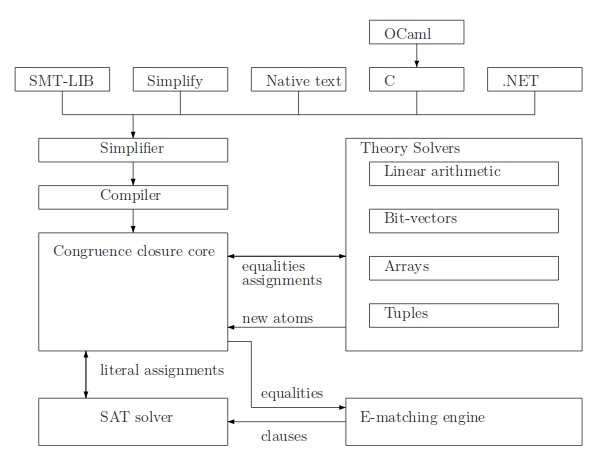
\includegraphics[width=1\textwidth]{arhitektura.png}
  \caption{Arhitektura rešavača Z3}
  \label{fig:arhitektura}
\end{figure}
\par
Formule prosleđene rešavaču se najpre procesiraju upotrebom simplifikacije. Simplifikacija primenjuje algebarska pravila redukcije kao što je \texttt{p $\land$ true $\vdash$ p}. Ovim procesom vrše se i odgovarajuće zamene kao što je \texttt{x=4 $\land$ q(x) $\vdash$ x=4 $\land$ q(4)}.
Nakon simplifikacije, kompajler formira apstraktno sintaksno stablo formula čiji su čvorovi simplifikovane formule (klauze). Zatim se jezgru kongruentnog zatvorenja (eng. 
\textit{Congruence closure core}) prosleđuje apstraktno sintaksno stablo. Jezgro kongruentnog zatvorenja komunicira sa SAT rešavačem koji određuje istinitosnu vrednost klauza. 
\par


Glavni gradivni blokovi formula su konstante, funkcije i relacije. Konstante su specijalan slučaj funkcija bez parametara. Svaka konstanta je određene sorte. Sorta odgovara tipu u programskim jezicima. Relacije su funkcije koje vraćaju povratnu vrednost tipa Boolean. Funkcije mogu uzimati argumente tipa Boolean pa se na taj način relacije mogu koristiti kao argumenti funkcija.  


Formula $F$ je validna ako je vrednost valuacije $true$ za bilo koje interpretacije funkcija i konstantnih simbola. Formula $F$ je zadovoljiva ukoliko postoji bar jedna valuacija u kojoj je formula tačna. Da bismo odredili da li je formula $F$ validna, rešavač Z3 proverava da li je formula $\lnot F$ zadovoljiva. Ukoliko je negacija formule nezadovoljiva, onda je polazna formula validna. 



\section{Teorije} \label{sec:num2}
Teorije rešavača Z3 su opisane u okviru višesortne logike prvog reda sa jednakošću.  Definisanjem specifične teorije, uvode se restrikcije pri definisanju formula kao i podržanih relacija i operatora koje se nad njima primenjuju. Na taj način, specijalizovane metode u odgovarajućoj teoriji mogu biti efikasnije implementirane u poređenju sa opštim slučajem. U nastavku će biti opisane teorija neinterpretiranih funkcija, teorija linearne aritmetike, teorija nelinearne aritmetike, teorija bitvektora i teorija nizova.

\subsection{Teorija neinterpretiranih funkcija}
Teorije obično određuju interpretaciju funkcijskih simbola. Teorija koja ne zadaje nikakva ograničenja za funkcijske simbole naziva se teorija neinterpretiranih funkcija 
(eng. \textit{Theory of Equality with Uninterpreted Functions}, skraćeno EUF). \par Kod rešavača Z3, funkcije i konstantni simboli su neinterpretirani. Ovo je kontrast u odnosu na funkcije odgovarajućih teorija. Funkcija + ima standardnu interpretaciju u teoriji aritmetike. Neinterpretirane funkcije i konstante su maksimalno fleksibilne i dozvoljavaju bilo koju interpretaciju koja je u skladu sa ograničenjima. Za razliku od programskih jezika, funkcije logike prvog reda su totalne, tj. definisane su za sve vrednosti ulaznih parametara. Na primer, deljenje 0 je dozvoljeno, ali nije specifikovano šta ono predstavlja. Teorija neinterpretiranih funkcija je odlučiva i postoji procedura odlučivanja polinomijalne vremenske složenosti. Jedna od procedura odlučivanja za ovu teoriju zasniva se na primeni algoritma Nelson-Open (eng. \textit{Nelson-Open algorithm}). O ovom algoritmu može se više naći u literaturi \cite{NelsonOpen}.
\par



\subsection{Teorija linearne aritmetike} 

Rešavač Z3 sadrži procedure odlučivanja za linearnu aritmetiku nad celobrojnim i realnim brojevima. Dodatni materijali o procedurama odlučivanja linearne aritmetike dostupni su u literaturi \cite{FastLinearArithmetic}.
\par

U okviru celobrojne linearne aritmetike, podržani funkcijski simboli su $+$, $-$ i $*$ pri čemu je kod množenja drugi operand konstanta. Nad funkcijskim simbolima, čiji su specijalni slučajevi konstante mogu se primenjivati relacijski operatori $<$, $\leq$, $>$ i $\geq$. 
\par
U okviru realne linearne aritmetike, podržani funkcijski simboli su $+$, $-$ i $*$ pri čemu je kod operacije množenja drugi operand konstanta. Pored ovih podržane su operacije $div$ i $mod$, uz uslov da je drugi operand konstanta različita od 0. Nad funkcijskim simbolima, čiji su specijalni slučajevi konstante mogu se primenjivati relacijski operatori $<$, $\leq$, $>$ i $\geq$. 
\par
\subsection{Teorija nelinearne aritmetike} 

Formula predstavlja formulu nelinearne aritmetike ako je oblika (* t s), pri čemu t i s nisu linearnog oblika.
Nelinearna celobrojna aritmetika je neodlučiva, tj. ne postoji procedura koja za proizvoljnu formulu vraća zadovoljivost ili nezadovoljivost. U najvećem broju slučajeva, Z3 vraća nepoznat rezultat. Za nelinearne probleme, rešavač Z3 koristi posebne metode odlučivanja zasnovane na Grebnerovim bazama. 


\subsection{Teorija bitvektora} 
Rešavač Z3 podržava bitvektore proizvoljne dužine. \texttt{(\_ BitVec n)} je sorta bitvektora čija je dužina \texttt{n}. Bitvektor literali se mogu definisati koristeći binarnu, decimalnu ili heksadecimalnu notaciju. U binarnom i heksadecimalnom slučaju, veličina bitvektora je određena brojem karaktera. Na primer, literal \textit{\#b010} u binarnom formatu je bitvektor dužine 3. Kako konstanta \textit{a} u heksadecimalnom formatu odgovara vrednosti 10, literal \textit{\#x0a} je bitvektor veličine 10. Veličina bitvektora mora biti specifikovana u decimalnom formatu. Na primer, reprezentacija \textit{(\_ bv10 32)} je bitvektor dužine 32 sa vrednošću 10. Podrazumevano, Z3 predstavlja bitvektore u heksadecimalnom formatu ukoliko je dužina bitvektora umnožak broja 4 a u suprotnom u binarnom formatu. Bitvektor literali mogu biti reprezentovani u decimalnom formatu. Više materijala o procedurama odlučivanja za teoriju bitvektora može se naći u literaturi \cite{DPBitvector}.

Pri korišćenju operatora nad bitvektorima, mora se eksplicitno navesti tip operatora. Zapravo, za svaki operator podržane su dve varijante za rad sa označenenim i neoznačenim operandima. Ovo je kontrast u odnosu na programske jezike u kojima kompajler na osnovu argumenata implicitno određuje tip operacije (označena ili neoznačena varijanta).
\par
U skladu sa prethodno navedenom činjenicom, teorija bitvektora ima na raspolaganju različite verzije aritmetičkih operacija za označene i neoznačene operande. Za rad sa bitvektorima od aritmetičkih operacija definisane su operacije sabiranja, oduzimanja, određivanje negacije (zapisivanja broja u komplementu invertovanjem svih bitova polaznog broja), množenja, izračunavanja modula pri deljenju, šiftovanje u levo kao i označeno i neoznačeno šiftovanje u desno. Podržane su sledeće logičke operacije: disjunkcija, konjunkcija, unarna negacija, negacija konjunkcije i negacija disjunkcije. Definisane su različite relacije nad bitvektorima kao što su $\leq$, $<$, $\geq$ i $>$.



\subsection{Teorija nizova} 
Osnovnu teoriju nizova karakterišu \texttt{select} i \texttt{store} funkcije. 
Funkcijom \texttt{(select a i)} vraća se vrednost na poziciji i u nizu a, dok se funkcijom \texttt{(store a i v)} formira novi niz, identičan nizu a pri čemu se na poziciji i nalazi vrednost v.
Z3 sadrži procedure odlučivanja za osnovnu teoriju nizova.
Dva niza su jednaka ukoliko su vrednosti svih elemenata na odgovarajućim pozicijama jednake.
 

\subsubsection{Konstantni nizovi}

Nizovi sa konstantnim vrednostima mogu se specifikovati koristeći \texttt{const} konstrukciju. Prilikom upotrebe \texttt{const} konstrukcije rešavač Z3 ne može da odluči kog tipa su elementi niza pa se on mora eksplicitno navesti. Interpretacija nizova je slična interpretaciji funkcija. Z3 koristi konstrukciju \texttt{(\_ as-array f)} za određivanje interpretacije niza. Ako je niz a jednak rezultatu konstrukcije \texttt{(\_ as-array f)}, tada za svaki indeks i, vrednost \texttt{(select a i)} odgovara vrednosti \texttt{(f i)}. 


\subsubsection{Primena map funkcije na nizove}
Rešavač Z3 obezbeđuje primenu parametrizovane funkcije \texttt{map} na nizove. Funkcijom \texttt{map} omogućava se primena proizvoljnih funkcija na sve elemente niza.

Nad nizovima se mogu vršiti slične operacije kao i nad skupovima. Rešavač Z3 ima podršku za računanje unije, preseka i razlike dva niza. Ovi operatori se tumače na isti način kao i u teoriji skupova. Za nizove a i b, pomenuti operatori mogu se koristiti navođenjem funkcija:\\
\texttt{(union a b)} ; kreiranje unije dva niza kao skupa \\
\texttt{(intersect a b)} ; kreiranje preseka dva niza kao skupa \\
\texttt{(difference a b)} ; kreiranje razlike dva niza kao skupa

\section{Tipovi podataka} \label{sec:num3}
U okviru rešavača Z3 dostupni su primitivni tipovi podataka, definisanjem konstanti različitih sorti. Neke od najčešće korišćenih su konstante bulovske, celobrojne i realne sorte.
Pored toga, mogu se definisati algebarski tipovi podataka. Algebarski tipovi podataka omogućavaju specifikaciju uobičajnih struktura podataka. Slogovi, torke i skalari (enumeracijski tipovi) spadaju u algebarske tipove podataka. Primena algebarskih tipova podataka može se generalizovati. Mogu se koristiti za specifikovanje konačnih listi, stabala i rekurzivnih struktura. 
\subsubsection{Slogovi}
Slog se specifikuje kao tip podataka sa jednim konstruktorom i proizvoljnim brojem elemenata sloga. Rešavač Z3 ne dozvoljava povećavanje broja argumenata sloga nakon njegovog definisanja. Važi svojstvo da su dva sloga jednaka samo ako su im svi argumenti jednaki.
\subsubsection{Skalari (tipovi enumeracije)}

Sorta skalara je sorta konačnog domena. Elementi konačnog domena se tretiraju kao različite konstante. Na primer, neka je S skalarni tip sa tri vrednosti A, B i C. Moguće je da tri konstante skalarnog tipa S budu različite. Ovo svojstvo ne može važiti u slučaju četiri konstante.


\subsubsection{Rekurzivni tipovi podataka}

Deklaracija rekurzivnog tipa podataka uključuje sebe direktno kao komponentu. Standardni primer rekurzivnog tipa podataka je lista. 
Lista celobrojnih vrednosti sa imenom \texttt{list} može se deklarisati naredbom:\\
\texttt{(declare-datatypes (list (nil) ((head Int) (tail list)))}
\par
Rešavaš Z3 ima ugrađenu podršku za liste korišćenjem ključne reči \texttt{List}.
Prazna lista se definiše korišćenjem klučne reči \texttt{nil} a konstruktor \texttt{insert} se koristi za dodavanje elemenata u listu. Selektori \texttt{head} i \texttt{tail} se definišu na uobičajan način.


\section{Upotreba rešavača korišćenjem SMT-LIB standarda} \label{sec:num4}
Ulazni format rešavača Z3 je definisan SMT-LIB 2.0 standardom \cite{SMTLIB}. Standard definiše jezik logičkih formula čija se zadovoljivost proverava u odnosu na neku teoriju. Cilj standarda je pojednostavljivanje jezika logičkih formula povećavanjem njihove izražajnosti i fleksibilnosti kao i obezbeđivanje zajedničkog jezika za sve SMT rešavače. 
\par
Interno, Z3 održava stek korisnički definisanih formula i deklaracija. Formule i deklaracije jednim imenom nazivamo tvrđenjima. Komandom \texttt{push} kreira se novi opseg i čuva se trenutna veličina steka. Komandom \texttt{pop} uklanjaju se sva tvrđenja i deklaracije zadate posle push-a sa kojim se komanda uparuje. Komandom \texttt{assert} dodaje se formula na interni stek. Skup formula na steku je zadovoljiv ako postoji interpretacija u kojoj sve formule imaju istinitosnu vrednost tačno. Ova provera se vrši komandom \texttt{check-sat}. U slučaju zadovoljivosti vraća se \texttt{sat}, u slučaju nezadovoljivosti vraća se \texttt{unsat} a kada rešavač ne može da proceni da li je formula zadovoljiva ili ne vraća se \texttt{unknown}. Komandom \texttt{get-model} vraća se interpretacija u kojoj su sve formule na steku tačne. 
\par

Komandom \texttt{declare-const} deklariše se konstanta odgovarajuće sorte. Sorta može biti parametrizovana i u tom slučaju su specifikovana imena njenih parametara. Naredbom \texttt{(define-sort [symbol] ([symbol]+)[sort])} vrši se specifikacija sorte.
Komandom \texttt{declare-fun} deklariše se funkcija. 
U primeru \ref{example1} koristimo činjenicu da se validnost formule pokazuje ispitivanjem zadovoljivosti negirane formule. 

\begin{primer} \label{example1} Dokazivanje de Morganovog zakona dualnosti\label{primer:demorgan} ispitivanjem validnosti formule: $\neg{(a \land b)} \Leftrightarrow (\neg{a} \lor \neg{b}) $ tako što se kao ograničenje dodaje negacija polazne formule. Z3 pronalazi da je negacija formule nezadovoljiva, pa je polazna formula tačna u svim interpretacijama. \\

\hspace{-0.6cm}
\begin{minipage}[b]{0.5\textwidth}
\textbf{Formula prosleđena rešavaču:}
\\(declare-const a Bool)
\\(declare-const b Bool)
\\(define-fun demorgan () Bool
\\\tab (= (and a b) (not (or (not a) (not b))))
\\)
\\(assert (not demorgan))
\\(check-sat) 
\\(get-model)
\end{minipage}
\hspace{1.5cm}
\begin{minipage}[t]{0.4\textwidth}
\vspace{-5.35cm}
\textbf{Izlaz:}
\\unsat
\end{minipage}
\end{primer}

Rešavač Z3 ima podršku za celobrojne i realne konstante. Komandom \texttt{declare-const} deklarišu se celobrojne i realne konstante. Rešavač ne vrši automatsku konverziju između celobrojnih i realnih konstanti. Ukoliko je potrebno izvršiti ovakvu konverziju koristi se funkcija \texttt{to-real} za konvertovanje celobrojnih u realne vrednosti.
Realne konstante treba da budu zapisane sa decimalnom tačkom. Primer \ref{example2} ilustruje deklarisanje konstanti i funkcija kao i primenu funkcije na konstante. Ispituje se zadovoljivost ograničenja.

\begin{primer} \label{example2} 
Rešavaču se prosleđuje ograničenja koje sadrže primenu funkcije f na celobrojnu konstantu a kao i relacijske operatore. Rešavač Z3 pronalazi da je ovo tvrđenje zadovoljivo i daje prikazani model. 
\\ 

\hspace{-0.7cm}
\begin{minipage}[b]{0.43\textwidth}
\textbf{Formula prosleđena rešavaču:}\\
(declare-const a Int)\\
(declare-fun f (Int Bool) Int)\\
(assert (> a 10))\\
(assert (< (f a true) 100))\\
(check-sat)\\
(get-model) \\
\end{minipage}
\hspace{0.6cm}
\begin{minipage}[t]{0.5\textwidth}
\vspace{-4.715cm}
\textbf{Izlaz:}
\\sat 
\\(model 
\\\tab(define-fun a () Int 11) 
\\\tab(define-fun f ((x!1 Int) (x!2 Bool)) Int 
\\\tab(ite (and (= x!1 11) (= x!2 true)) 0 0))
\\)
\end{minipage}
\end{primer}

Primer \ref{example3} ilustruje pronalaženje interpretacija celobrojnih i realnih konstanti. Interpretacija se svodi na pridruživanje brojeva svakoj konstanti. 

\begin{primer} \label{example3} 
Rešavaču se prosleđuju jednostavna ograničenja za celobrojne i realne konstante.
Ograničenja sadrže aritmetičke i relacijske operatore. Rešavač vraća zadovoljivost tvrđenja i dobijeni model prikazujemo u nastavku.\\ \\
\begin{minipage}[b]{0.47\textwidth}
\textbf{Formula prosleđena rešavaču:}
\\(declare-const a Int)
\\(declare-const b Int)
\\(declare-const c Int)
\\(declare-const d Real)
\\(declare-const e Real)
\\(assert (> e (+ (to\_real (+ a b)) 2.0)))
\\(assert (= d (+ (to\_real c) 0.5)))
\\(check-sat)
\\(get-model)
\end{minipage}
\hspace{1.6cm}
\begin{minipage}[t]{0.4\textwidth}
\vspace{-6cm}
\textbf{Izlaz:}
\\sat 
\\(model
\\\tab(define-fun b () Int 0) 
\\\tab(define-fun a () Int 1) 
\\\tab(define-fun e () Real 4.0) 
\\\tab(define-fun c () Int 0) 
\\\tab(define-fun d () Real (/ 1.0 
\\\tab 2.0))
\\)
\end{minipage}

\end{primer}


Takođe, postoji uslovni operator (if-then-else operator). Na primer,
izraz (ite (and (= x!1 11) (= x!2 false)) 21 0) ima vrednost 21 kada je promenljiva x!1 jednaka 11, a promenljiva x!2 ima vrednost False. U suprotnom, vraća se 0.

U slučaju deljenja, može se koristiti \texttt{ite} (if-then-else) operator i na taj način se može dodeliti interpretacija u slučaju deljenja nulom.
\par
Mogu se konstruisati novi operatori, korišćenjem \texttt{define-fun} konstruktora. Ovo je zapravo makro, pa će rešavač vršiti odgovarajuće zamene. U primeru \ref{example4} ilustruje se definisanje novog operatora. Zatim se novi operator primenjuje na konstante, uvode se ograničenja i ispituje njihova zadovoljivost.
\begin{primer} \label{example4}
Definišemo operator deljenja tako da rezultat bude specifikovan i kada je delilac 0. Uvode se dve konstante realnog tipa i primenjuje se definisani operator. Z3 rešavač pronalazi nezadovoljivost tvrđenja s obzirom da operator \texttt{mydiv} vraća 0 pa relacija poređenja ne može biti tačna.\\ \\
\begin{minipage}[b]{0.5\textwidth}
\textbf{Formula prosleđena rešavaču:}
\\(define-fun mydiv ((x Real) (y Real)) Real
\\\tab (if (not (= y 0.0))  (/ x y)  0.0))
\\(declare-const a Real)
\\(declare-const b Real)
\\(assert (>= (mydiv a b) 1.0))
\\(assert (= b 0.0))
\\(check-sat)
\end{minipage}
\hspace{3cm}
\begin{minipage}[t]{0.4\textwidth}
\vspace{-4.73cm}
\textbf{Izlaz:}
\\unsat
\end{minipage}
\end{primer}
\par
Primer \ref{example5} ilustruje rešavanje nelinearnog problema uvođenjem ograničenja nad realnim konstantama. Ispituje se zadovoljivost prosleđenih ograničenja. Kada su prisutna samo nelinearna ograničenja nad realnim konstantama, Z3 koristi posebne metode odlučivanja,
\begin{primer} \label{example5} Rešavaču se prosleđuje ograničenja $b^{3} + b*c = 3$ nad realnim konstantama. Rešavač vraća zadovoljivost tvrđenja i dobijeni model prikazujemo u nastavku.   
\\ \\
\begin{minipage}[b]{0.43\textwidth}
\textbf{Formula prosleđena rešavaču:}
\\(declare-const b Real)
\\(declare-const c Real)
\\(assert (= (+ (* b b b) (* b c)) 3.0))
\\(check-sat)
\\(get-model)

\end{minipage}
\hspace{1.5cm}
\begin{minipage}[t]{0.45\textwidth}
\vspace{-3.4cm}
\textbf{Izlaz:}
\\sat 
\\(model 
\\\tab(define-fun b () Real (/ 1.0 8.0)) 
\\\tab(define-fun c () Real (/ 15.0 64.0))
\\)
\end{minipage}
\end{primer}
\par
Primer \ref{example6} ilustruje različite načine predstavljanja bitvektora. Ukoliko zapis počinje sa \#b, bitvektor se zapisuje u binarnom formatu. Ukoliko zapis počinje sa \#x, bitvektor se zapisuje u heksadecimalnom formatu.
\begin{primer} \label{example6} 
Nakon specifikacije formata, zapisuje se dužina vektora. Drugi način zapisa počinje skraćenicom \texttt{bv}, navođenjem vrednosti i na kraju dužine. Komandom \texttt{(display t)} štampa se izraz \texttt{t}.\\\\
\begin{minipage}[b]{0.45\textwidth}
\textbf{Formula prosleđena rešavaču:}
\\(display \#b0100)
\\(display (\_ bv20 8))
\\(display (\_ bv20 7))
\\(display \#x0a) 
\\(set-option :pp.bv-literals false)
\\(display \#b0100)
\\(display (\_ bv20 8))
\\(display (\_ bv20 7))
\\(display \#x0a)
\end{minipage}
\hspace{2.5cm}
\begin{minipage}[t]{0.4\textwidth}
\vspace{-5.93cm}
\textbf{Izlaz:}
\\\#x4 
\\\#x14 
\\\#b0010100 
\\\#x0a 
\\(\_ bv4 4) 
\\(\_ bv20 8) 
\\(\_ bv20 7) 
\\(\_ bv10 8)
\end{minipage}
\end{primer}
\par Primer \ref{example7} ilustruje primenu aritmetičkih operacija nad bitvektorima. Podržane aritmetičke operacije su sabiranje \texttt{(bvadd)}, oduzimanje \texttt{(bvsub)}, unarna negacija \texttt{(bvneg)}, množenje \texttt{(bvmul)}, računanje modula \texttt{(bvmod)}, šiftovanje ulevo \texttt{(bvshl)}, neoznačeno (logičko) šiftovanje udesno \texttt{(bvlshr)} i označeno (aritmetičko) šiftovanje udesno \texttt{(bvashr)}. Od logičkih operacija postoji podrška za disjunkciju \texttt{(bvor)}, konjunkciju \texttt{(bvand)}, ekskluzivnu disjunkciju \texttt{(bvxor)}, negaciju disjunkcije \texttt{(bvnor)}, negaciju konjunkcije \texttt{(bvnand)} i negaciju ekskluzivne disjunkcije \texttt{(bvnxor)}.
\begin{primer} \label{example7} 
Ovaj primer ilustruje primenu nekih aritmetičkih operacija nad bitvektorima i dobijene rezultate. Komandom \texttt{(simplify t)} prikazuje se jednostavniji izraz ekvivalentan izrazu \texttt{t} ukoliko postoji.
\\ \\
\begin{minipage}[b]{0.5\textwidth}
\textbf{Formula prosleđena rešavaču:}
\\(simplify (bvadd \#x07 \#x03)) 
\\(simplify (bvsub \#x07 \#x03)) 
\\(simplify (bvneg \#x07))       
\\(simplify (bvmul \#x07 \#x03)) 
\\(simplify (bvsmod \#x07 \#x03)) 
\\(simplify (bvshl \#x07 \#x03)) 
\\(simplify (bvlshr \#xf0 \#x03))  
\\(simplify (bvashr \#xf0 \#x03))  
\\(simplify (bvor \#x6 \#x3)) 
\\(simplify (bvand \#x6 \#x3))   
\end{minipage}
\hspace{2.5cm}
\begin{minipage}[b]{0.5\textwidth}
\textbf{Izlaz:}
\\\#x0a 
\\\#x04 
\\\#xf9 
\\\#x15 
\\\#x01 
\\\#x38 
\\\#x1e 
\\\#xfe
\\\#x7 
\\\#x2 
\end{minipage}

\end{primer} \par
Postoji brz način da se proveri da li su brojevi fiksne dužine stepeni dvojke. U primeru \ref{example8} pokazuje se da je bitvektor x stepen dvojke ako i samo ako je vrednost izraza x $\land$ (x - 1) jednaka 0.

\begin{primer} \label{example8}
Provera da li je broj stepen dvojke primenjuje se na bitvektore čije su vrednosti 0, 1, 2, 4 i 8. Rešavaču se prosleđuje negacija formule. U svim slučajevima brojevi su stepeni dvojke pa Z3 rešavač vraća nezadovoljivost.\\ \\
\begin{minipage}[b]{0.5\textwidth}
\textbf{Formula prosleđena rešavaču:}
\\(define-fun is-power-of-two 
\\\tab((x (\_ BitVec 4))) Bool 
\\\tab(= \#x0 (bvand x (bvsub x \#x1)))
\\)
\\(declare-const a (\_ BitVec 4))
\\(assert 
\\\tab(not (= (is-power-of-two a) 
\\\tab\tab    (or (= a \#x0) 
\\\tab\tab\tab     (= a \#x1) 
\\\tab\tab\tab     (= a \#x2) 
\\\tab\tab\tab     (= a \#x4) 
\\\tab\tab\tab     (= a \#x8)
\\\tab\tab		))
\\\tab )
\\)
\\(check-sat)
\end{minipage}
\hspace{2.5cm}
\begin{minipage}[t]{0.5\textwidth}
\vspace{-10.45cm}
\textbf{Izlaz:}
\\unsat
\end{minipage}
\end{primer}
\par Primer \ref{example9} ilustruje upotrebu relacija nad bitvektorima. Podržane relacije uključuju neoznačene i označene verzije za operatore $<$, $\leq$, $>$ i $\geq$. Neoznačene varijante počinju nazivom \texttt{bvu}, a u nastavku sledi ime relacije. Označene varijante počinju nazivom \texttt{bvs}, a u nastavku ponovo sledi ime relacije. 
\begin{primer} \label{example9} Primer ilustruje upotrebu označenih i neoznačenih verzija operatora nad bitvektorima. Na primer, relacija $\leq$ nad neoznačenim brojevima zadaje se komandom \texttt{bvule}, a relacija $>$ nad neoznačenim brojevima komandom \texttt{bvugt}. Slično, relacija $\geq$ nad neoznačenim brojevima zadaje se komandom \texttt{bvsge}, a relacija $<$ nad označenim brojevima komandom \texttt{bvslt}.
\\ \\ 
\begin{minipage}[b]{0.5\textwidth}
\textbf{Formula prosleđena rešavaču:}
\\(simplify (bvule \#x0a \#xf0))  
\\(simplify (bvult \#x0a \#xf0))  
\\(simplify (bvuge \#x0a \#xf0))  
\\(simplify (bvugt \#x0a \#xf0))  
\\(simplify (bvsle \#x0a \#xf0)) 
\\(simplify (bvslt \#x0a \#xf0))  
\\(simplify (bvsge \#x0a \#xf0))  
\\(simplify (bvsgt \#x0a \#xf0))

\end{minipage}
\hspace{2cm} 
\begin{minipage}[t]{0.5\textwidth}
\vspace{-5.3cm}
\textbf{Izlaz:}
\\true 
\\true 
\\false 
\\false 
\\false 
\\false 
\\true 
\\true
\end{minipage}


\end{primer}

Rešavač Z3 nudi funkcije za promenu načina reprezentacije brojeva. Moguće su konverzije reprezentacije brojeva linearne aritmetike u reprezentaciju bitvektora i obrnuto. Ovaj rezultat može se postići naredbama: \\
\texttt{(define b (int2bv[32] z))} \\  
\texttt{(define c (bv2int[Int] x))}
\par
Primer \ref{example10} ilustruje poređenje bitvektora koristeći označene i neoznačene verzije operatora. Ispituje se zadovoljivost prosleđenog ograničenja.
\begin{primer} \label{example10} Označeno poređenje, kao što je bvsle, uzima u obzir znak bitvektora za poređenje, dok neoznačeno poređenje komandom bvule tretira bitvektor kao prirodan broj. Z3 rešavač pronalazi da je tvrđenje zadovoljivo i daje prikazani model.
\\ \\
\begin{minipage}[b]{0.5\textwidth}
\textbf{Formula prosleđena rešavaču:}
\\(declare-const a (\_ BitVec 4))
\\(declare-const b (\_ BitVec 4))
\\(assert (not (= (bvule a b) (bvsle a b)))
\\(check-sat)
\\(get-model)
\end{minipage}
\hspace{1.15cm} 
\begin{minipage}[t]{0.5\textwidth}
\vspace{-3.45cm}
\textbf{Izlaz:}
\\sat 
\\(model 
\\\tab(define-fun b () (\_ BitVec 4) \#xe) 
\\\tab(define-fun a () (\_ BitVec 4) \#x0)
\\)
\end{minipage}
\end{primer}
\par
Primer \ref{example11} ilustruje kako se definišu nizovi sa konstantnim vrednostima. Zatim se dodaju ograničenja korišćenjem funkcije \texttt{select} i ispituje se njihova zadovoljivost.
\begin{primer} \label{example11} Definišemo konstantni niz m celobrojnog tipa i dve celobrojne konstante a i i. Uvodimo ograničenje da niz m sadrži samo jedinice. Z3 pronalazi da je ovo tvrdjenje zadovoljivo i daje prikazani model.\\
\begin{minipage}[b]{0.55\textwidth}
\vspace{0.5cm} 
\textbf{Formula prosleđena rešavaču:}
\\(declare-const m (Array Int Int))
\\(declare-const a Int)
\\(declare-const i Int)
\\(assert (= m ((as const (Array Int Int)) 1)))
\\(assert (= a (select m i)))
\\(check-sat)
\\(get-model)
\end{minipage}
\hspace{1.1cm} 
\begin{minipage}[t]{0.5\textwidth}
\vspace{-4.7cm}
\textbf{Izlaz:}
\\sat 
\\(model 
\\\tab(define-fun m () (Array Int Int) 
\\\tab\tab(\_ as-array k!0)
\\\tab) 
\\\tab(define-fun i () Int 0) 
\\\tab(define-fun a () Int 1) 
\\\tab(define-fun k!0 ((x!0 Int)) 
\\\tab\tab Int (ite (= x!0 0) 1 1)
\\\tab)
\\)
\end{minipage}
\end{primer}
\par
Primer \ref{example12} ilustruje primenu funkcije \texttt{map} na sve elemente konstatnih nizova. Za svaka dva elementa koji pripadaju različitim nizovima, pokazuje se važenje De Morganovog zakona iz primera \ref{example1}. 
\begin{primer} \label{example12} 
Kao ograničenje dodajemo negaciju navedene formule. Rešavač Z3 vraća nezadovoljivost negirane formule, odakle zaključujemo da je polazna formula validna.\\ \\
\begin{minipage}[b]{0.65\textwidth}
\textbf{Formula prosleđena rešavaču:}
\\(define-sort Set (T) (Array T Bool))
\\(declare-const a (Set Int))
\\(declare-const b (Set Int))
\\(assert (not (= ((\_ map and) a b) ((\_ map not) 
\\\tab((\_ map or) ((\_ map not) b) ((\_ map not) a)))))
\\)
\\(check-sat)
\end{minipage}
\hspace{2.5cm} 
\begin{minipage}[t]{0.5\textwidth}
\vspace{-4.65cm}
\textbf{Izlaz:}
\\unsat 
\end{minipage}
\end{primer}

\par
U primeru \ref{example13} pokazuje se da su dva sloga jednaka ako i samo ako su im svi argumenti jednaki. Uvodi se parametarski tip \texttt{Pair} i koriste se selektorske funkcije \texttt{first} i \texttt{second}. 

\begin{primer} \label{example13} Nakon definisanja slogova p1 i p2, dodaje se ograničenje koje se odnosi na drugi element sloga.
Dodajemo i ograničenje da su slogovi p1 i p2 jednaki. Rešavač Z3 vraća zadovoljivost formule i odgovarajući model. 
\\ \\
\begin{minipage}[b]{0.5\textwidth}
\textbf{Formula prosleđena rešavaču:}
\\(declare-datatypes (T1 T2) 
\\\tab[0.3cm](Pair (mk-pair (first T1) (second T2))))
\\(declare-const p1 (Pair Int Int))
\\(declare-const p2 (Pair Int Int))
\\(assert (= p1 p2))
\\(assert (> (second p1) 20))
\\(check-sat)
\\(get-model)
\end{minipage}
\hspace{1.5cm} 
\begin{minipage}[t]{0.5\textwidth}
\vspace{-5.35cm}
\textbf{Izlaz:}
\\sat 
\\(model 
\\\tab(define-fun p1 () (Pair Int Int) 
\\\tab\tab(mk-pair 0 21)
\\\tab) 
\\\tab(define-fun p2 () (Pair Int Int) 
\\\tab\tab(mk-pair 0 21)
\\\tab)
\end{minipage}

\end{primer}
\par
U primeru \ref{example14} ilustruje se definisanje listi kao i dodavanje ograničenja korišćenjem selektorskih funkcija \texttt{head} i \texttt{tail}. Ispituje se zadovoljivost tvrđenja.
\begin{primer} \label{example14}
Pored ograničenja za prve elemente liste, tražimo model takav da liste l1 i l2 nisu jednake, tj. da nisu svi elementi na odgovarajućim pozicijama u listama jednaki. Rešavač Z3 vraća zadovoljivost tvrđenja i dobijeni model prikazujemo u nastavku.
\\ \\
\begin{minipage}[b]{0.42\textwidth}
\textbf{Formula prosleđena rešavaču:}
\\(declare-const l1 (List Int))
\\(declare-const l2 (List Int))
\\(declare-const l3 (List Int))
\\(declare-const x Int)
\\(assert (not (= l1 nil)))
\\(assert (not (= l2 nil)))
\\(assert (= (head l1) (tail l2)))
\\(assert (not (= l1 l2)))
\\(assert (= l3 (insert x l2)))
\\(assert (> x 100))
\\(check-sat)
\\(get-model)
\end{minipage}
\hspace{0.9cm}
\begin{minipage}[t]{0.55\textwidth}
\vspace{-7.84cm}
\textbf{Izlaz:}
\\sat 
\\(model 
\\\tab(define-fun l3 () (List Int) 
\\\tab(insert 101 (insert 0 (insert 1 nil)))
\\\tab(define-fun x () Int 101) 
\\\tab(define-fun l1 () (List Int) (insert 0 nil)) 
\\\tab(define-fun l2 () (List Int) (insert 0 
\\\tab\tab(insert 1 nil))
\\\tab)
\\) 
\end{minipage}


\end{primer}

U prethodnom primeru, uvode se ograničenja da su liste l1 i l2 različite od \texttt{nil}. Vrši se uvođenje ovih ograničenja jer interpretacija selektora \texttt{head} i \texttt{tail} 
nije specifikovana u slučaju praznih lista.



\section{Upotreba rešavača korišćenjem C++ interfejsa} \label{sec:num5}
C++ interfejs prema rešavaču Z3 obezbeđuje različite strukture podataka, klase i funkcije koje su potrebne za direktnu komunikaciju C++ aplikacije sa rešavačem. Neke od najbitnijih klasa biće opisane u nastavku, dok se kompletan opis interfejsa može naći na internetu \cite{cppapi}.

Klasa \texttt{Z3\_sort} koristi se za definisanje sorte izraza.  Prilikom definisanja izraza navodi se sorta kako bi bio poznat skup vrednosti koje mu se mogu dodeliti kao i skup dozvoljenih metoda. Sorte izraza definisane su tipom enumeracije. Neke od najvažnijih sorti su \texttt{Z3\_BOOL\_SORT}, \texttt{Z3\_INT\_SORT}, \texttt{Z3\_REAL\_SORT}, \texttt{Z3\_BV\_SORT} i \texttt{Z3\_ARRAY\_SORT}. Određivanje sorte izraza vrši se funkcijom \texttt{sort\_kind()} sa povratnom vrednošću tipa enumeracije. Za proveru pripadnosti izraza sorti, koriste se funkcije \texttt{is\_bool()}, \texttt{is\_int()}, \texttt{is\_real()}, \texttt{is\_array()} i \texttt{is\_bv()}. Sorte različitih izraza se mogu porediti korišćenjem operatora jednakosti. \par 

Za upravljanje objektima interfejsa kao i za globalno konfigurisanje koristi se klasa \texttt{context}. Klasa sadrži konstruktor bez argumenata. Upotrebom klase \texttt{context}, mogu se detektovati različite vrste grešaka u korišćenju C++ API-ja. Greške su definisane tipom enumeracije \texttt{Z3\_ERROR\_CODE}. Neke od konstanti enumeracije su \texttt{Z3\_OK}, \texttt{Z3\_SORT\_ERROR}, \texttt{Z3\_INVALID\_USAGE} i \texttt{Z3\_INTERNAL\_FATAL}.  Kontekst omogućava kreiranje konstanti metodama \texttt{bool\_const()}, \texttt{int\_const()}, \texttt{real\_const()} i \texttt{bv\_const()}. Definisanje različitih sorti omogućeno je metodama \texttt{bool\_sort()}, \texttt{int\_sort()}, \texttt{real\_sort()}, \texttt{bv\_sort()} i \texttt{array\_sort()}. 
\par

Izrazi koji se formiraju pripadaju klasi \texttt{expr}. Sadrži konstruktor čiji je argument objekat klase \texttt{context}. Za dobijanje izraza na zadatoj poziciji u skupu izraza koristi se metoda \texttt{at(expr const \&index)}.  Provera da li podizraz predstavlja deo drugog izraza vrši se metodom  \texttt{contains(expr const \&s)}. Za dobijanje pojednostavljenog izraza ekvivalentnog polaznom koristi se metoda \texttt{simplify()} ukoliko takav izraz postoji. Za dobijanje pojednostavljenog izraza može se navesti i skup parametara koji se prosleđuju Z3 simplifikatoru. Zamenu vektora izraza drugim vektorom vrši se metodom \texttt{substitute(expr\_vector const \&source, expr\_vector const \&destination)}. 
\par
Postoji veliki broj metoda i operatora koji se koriste za izgradnju složenih izraza. Podržan je veliki broj aritmetičkih operatora za rad za izrazima uključujući operatore sabiranja, oduzimanja, množenja, deljenja, računanja stepena i modula. Svi aritmetički operatori kao argumente imaju izraze. Rezultat primene operatora je novi izraz. Pored toga, mogu se koristiti i različiti logički operatori. Neke od podržanih logičkih operacija su konjunkcija, disjunkcija, implikacija, negacija konjunkcije i negacija disjunkcije. Konjunkcija vektora izraza vrši se metodom \texttt{mk\_and(expr\_vector const \&args)}. Disjunkcija vektora izraza vrši se metodom \texttt{mk\_or(expr\_vector const \&args)}. Implikacija dva izraza vrši se metodom \texttt{implies(expr const \&a, expr const \&b)}. Negacija konjunkcije dva izraza vrši se metodom \texttt{nand(expr const  \&a, expr const \&b)}. Negacija disjunkcije dva izraza vrši se metodom \texttt{nor(expr const \&a, expr const \&b)}. Nad izrazima se mogu primenjivati relacijski operatori \texttt{==}, \texttt{!=}, \texttt{<}, \texttt{<=}, \texttt{>}, \texttt{>=} pri čemu izrazi moraju biti odgovarajuće sorte kako bi poređenje bilo moguće. Nadovezivanje dva izraza vrši se metodom \texttt{concat(expr const \&a, expr const \&b)}. Može se vršiti i nadovezivanje vektora izraza. Kombinovanjem pomenutih metoda i operatora mogu se graditi izrazi proizvoljne složenosti. 	
\par
Definicija funkcije vrši se objektima klase \texttt{func\_decl}. Korišćenjem ove klase definišu se interpretirane i neinterpretirane funkcije rešavača Z3. 
Povratne vrednosti funkcija određene su tipom enumeracije \texttt{Z3\_decl\_kind}. Neke od konstanti enumeracije su \texttt{Z3\_OP\_TRUE}, \texttt{Z3\_OP\_FALSE}, \texttt{Z3\_OP\_REAL}, \texttt{Z3\_OP\_INT} i \texttt{Z3\_OP\_ARRAY}. Dobijanje imena funkcijskog simbola vrši se metodom \texttt{name()}. Određivanje arnosti funkcijskog simbola vrši se metodom \texttt{arity()}. Određivanje sorte i-tog parametra funkcijskog simbola određuje se metodom \texttt{domain(unsigned i)}. 
\par


U okviru C++ interfejsa, teorije rešavača Z3 zadate su semantički navođenjem modela. Ova podrška implementirana je klasom \texttt{model}. Sadrži konstruktor čiji je argument objekat klase \texttt{context}. Interpretacija izraza definisanog u modelu dobija se korišćenjem metode \texttt{eval(expr const \&n)}. Metodom \texttt{get\_func\_decl(unsigned i)} dobija se i-ti funkcijski simbol modela.  
Metodom \texttt{get\_const\_decl(unsigned i)} dobija se interpretacija i-te konstante modela. Metodom \texttt{num\_consts()} dobija se broj konstanti datog modela kao funkcijskih simbola arnosti 0. Metodom \texttt{num\_funcs()} dobija se broj funkcijskih simbola arnosti veće od 0.  Metodom \texttt{size()} vraća se broj funkcijskih simbola modela. Poređenje modela vrši se operatorom jednakosti. Dva modela su jednaka ukoliko su im jednake interpretacije svih funkcijskih simbola. Za ispisivanje modela, koristi se funkcija \texttt{Z3\_model\_to\_string} čiji su argumenti objekti klasa \texttt{context} i \texttt{model}.\par 


Sa Z3 rešavačem komunicira se korišćenjem objekta klase \texttt{solver}. Objekat klase \texttt{solver} inicijalizuje se vrednostima objekta klase \texttt{context}. Osnovni metodi klase solver su \texttt{add}, \texttt{check} i \texttt{get\_model}. Metodom \texttt{add(expr const \&e)} dodaje se ograničenje koje se prosleđuje rešavaču. Metodom \texttt{check()} proverava se zadovoljivost ograničenja prosleđenih rešavaču. Metodom \texttt{get\_model()} vraća se model definisan ograničenjima ukoliko postoji. Pre korišćenja metode \texttt{get\_model()}, mora se pozvati metod \texttt{check()}. Metodom \texttt{assertions()} vraća se vektor ograničenja prosleđenih rešavaču. Ograničenja se mogu čitati iz fajla i iz stringa, korišćenjem metoda \texttt{from\_file(char const *file)} i \texttt{from\_string(char const *s)}. Uklanjanje svih ograničenja prosleđenih rešavaču vrši se metodom \texttt{reset()}. \par

\subsection{Interfejs kroz primere}
Naredni primeri ilustruju korišćenje najvažnijih klasa i metoda C++ interfejsa za komunikaciju sa Z3 rešavačem. Primer \ref{ex1} ilustruje kreiranje bulovskih izraza i jednostavne formule i prikazuje kako se kreira i upotrebljava klasa \texttt{context} i klasa \texttt{solver}. U ovom primeru, ilustrovano je dodavanje ograničenja u solver metodom \texttt{add} i proveravanje njegove zadovoljivosti metodom \texttt{check}. 

\begin{primer} \label{ex1} Primer demonstrira važenje De Morganovog zakona dokazivanjem formule iz primera \ref{primer:demorgan}. Pokazuje se nezadovoljivost negirane formule. U zavisnosti od rezultata štampa se odgovarajuća poruka.
\begin{lstlisting}[language=C++]
void demorgan() {
    context c;
    expr x = c.bool_const("x");
    expr y = c.bool_const("y");
    expr e = (!(x && y)) == (!x || !y);
    
    solver s(c);
    s.add(!e);

    switch (s.check()) {
    case unsat:   std::cout << "Formula je validna"; break;
    case sat:     std::cout << "Formula nije validna"; break;
    case unknown: std::cout << "Rezultat je nepoznat"; break;
    }
}
\end{lstlisting}
\end{primer}

Primer \ref{ex2} ilustruje kreiranje celobrojnih konstanti i jednostavne neinterpretirane funkcije upotrebom klase \texttt{func\_decl}. Prilikom definisanja funkcije navodi se njeno ime kao i sorte argumenta i povratne vrednosti. Ilustruje se kreiranje složenijeg izraza upotrebom metode \texttt{implies} koji odgovara logičkom operatoru implikacije. Složeniji izraz prosleđuje se solveru i proverava se njegova zadovoljivost.
\begin{primer} \label{ex2} Primer demonstrira upotrebu neinterpretiranih funkcija dokazivanjem formule x = y => g(x) = g(y). Dodaje se negacija prethodno navedene formule. U zavisnosti od rezultata, štampa se odgovarajuća poruka.\\
\begin{lstlisting}[language=C++]
void primer_sa_neinterpretiranim_funkcijama() { 
    context c;
    expr x      = c.int_const("x");
    expr y      = c.int_const("y");
    sort I      = c.int_sort();
    func_decl g = function("g", I, I);
    
    solver s(c);
    expr e = implies(x == y, g(x) == g(y));
    s.add(!e);
    if (s.check() == unsat) 
        std::cout << "dokazano";
    else
        std::cout << "nije dokazano";
}
\end{lstlisting}
\end{primer}
U primeru \ref{ex3} korišćenjem metode \texttt{get\_model} pristupa se modelu koji je solver vratio. Vrši se evaluacija izraza dobijenih iz modela primenom metode \texttt{eval}.  
\begin{primer} \label{ex3} Rešavaču se prosleđuju jednostavna ograničenja nad konstantama. Zatim se vrši evaluacija jednostavnih izraza nad konstantama definisanih u modelu.
\begin{lstlisting}[language=C++]
void eval_primer() {
    context c;
    expr x = c.int_const("x");
    expr y = c.int_const("y");
    solver s(c);

    s.add(x < y);
    s.add(x > 2);
    std::cout << s.check();
    
    model m = s.get_model();
    std::cout << "Model:" << m;
    std::cout << "x+y = " << m.eval(x+y);
}
\end{lstlisting}
\end{primer}


Primer \ref{ex4} ilustruje pronalaženje interpretacija konstanti modela za problem linearne aritmetike uvođenjem ograničenja.
Pokazuje se kako se korišćenjem klase \texttt{func\_decl} pristupa konstantama modela kao funkcijskim simbolima arnosti 0.
\begin{primer} \label{ex4}
Rešavaču se prosleđuju jednostavna ograničenja linearne aritmetike $x >= 1$  i $y < x + 3$. Ispisuju se imena i interpretacije konstanti modela korišćenjem
funkcije \texttt{arity} klase \texttt{func\_decl}.
\\
\begin{lstlisting}[language=C++]
void primer_linearne_aritmetike() {
    context c;
    expr x = c.int_const("x");
    expr y = c.int_const("y");
    solver s(c);
    s.add(x >= 1);
    s.add(y < x + 3);
    model m = s.get_model();

    for(unsigned i = 0; i < m.size(); i++) {
        func_decl v = m[i];
        assert(v.arity() == 0); 
        std::cout << v.name() << "=" << m.get_const_interp(v);
    }
}
\end{lstlisting}
\end{primer}

Primer \ref{ex5} ilustruje pronalaženje interpretacija realnih konstanti modela za problem nelinearne aritmetike uvođenjem ograničenja. Interpretacija realnih konstanti ispisuje se u celobrojnom i realnom formatu korišćenjem opcija za konfigurisanje formata ispisa klase \texttt{context}. 

\begin{primer} \label{ex5}
Rešavaču se prosleđuju jednostavna ograničenja nelinearne aritmetike 
$x^2 + y^2 = 1$ i $x^3 + z^3 < 0.5$. Ispisuju se imena i interpretacije konstanti modela korišćenjem funkcije \texttt{arity} klase \texttt{func\_decl}.
\\
\begin{lstlisting}[language=C++]
void primer_nelinearne_aritmetike() {    
    context c;
    expr x = c.real_const("x");
    expr y = c.real_const("y");
    expr z = c.real_const("z");
                     
    solver s(c);
    s.add(x*x + y*y == 1);                    
    s.add(x*x*x + z*z*z < c.real_val("1/2"));  
    
    std::cout << s.check();
    model m = s.get_model();
    std::cout << m;
    
    for(unsigned i = 0; i < m.size(); i++) {
        func_decl v = m[i];
        assert(v.arity() == 0); 
        std::cout << v.name() << "=" << m.get_const_interp(v);
    }

}
\end{lstlisting}
\end{primer}


Primer \ref{ex6} ilustruje pronalaženje interpretacija konstanti koje imaju bitvektorsku reprezentaciju korišćenjem metode \texttt{bv\_const} klase \texttt{context}. Parametri ove metode su ime i broj mesta za zapisivanje konstante. 
\begin{primer} \label{ex6} 
Rešavaču se prosleđuje ograničenje $x^y - 103 = x*y$. 
Ispisuju se imena i interpretacije konstantni predstavljenih bitvektorom dužine 32 korišćenjem funkcije \texttt{arity} klase \texttt{func\_decl}.
\begin{lstlisting}[language=C++]
void primer_sa_bitvektorima() {
    context c;
    expr x = c.bv_const("x", 32);
    expr y = c.bv_const("y", 32);

    solver s(c);
    s.add((x ^ y) - 103 == x * y);
    std::cout << s.check();
    std::cout << s.get_model();
    
    for(unsigned i = 0; i < m.size(); i++) {
        func_decl v = m[i];
        assert(v.arity() == 0); 
        std::cout << v.name() << "=" << m.get_const_interp(v);
    }
}

\end{lstlisting}
\end{primer}



------------------------------------------------------------------------------

% ------------------------------------------------------------------------------
\chapter{Zaključak}
% ------------------------------------------------------------------------------


% ------------------------------------------------------------------------------
% Literatura
% ------------------------------------------------------------------------------
\literatura

% ==============================================================================
% Završni deo teze i prilozi
\backmatter
% ==============================================================================

% ------------------------------------------------------------------------------
% Biografija kandidata
\begin{biografija}
  
\end{biografija}
% ------------------------------------------------------------------------------

\end{document}
